\documentclass{article}
\usepackage{graphicx}
\usepackage{color}
\usepackage{amssymb}
\usepackage{amsmath}
\usepackage{multirow}
\usepackage{multicol}
\usepackage{array}
\usepackage{rotating,capt-of}
\usepackage[small]{caption}
\usepackage{booktabs}
%\usepackage{float} % for placing figures where i want
\usepackage{afterpage}
\usepackage{epsfig, a4wide}

\usepackage{tikz,graphicx}
\usetikzlibrary{shapes.geometric, arrows}
\usetikzlibrary{shapes.misc, positioning}
\usetikzlibrary{backgrounds}

\definecolor{lavander}{cmyk}{0,0.48,0,0}
\definecolor{violet}{cmyk}{0.79,0.88,0,0}
\definecolor{burntorange}{cmyk}{0,0.52,1,0}

\def\lav{lavander!90}
\def\oran{orange!30}

\tikzstyle{neighbors}=[draw,circle,violet,bottom color=\lav,
                  top color= white, font=\scriptsize,text=violet,minimum width=10pt]
\tikzstyle{queries}=[draw,circle,burntorange, left color=\oran,
                       text=violet,minimum width=30pt]

\tikzstyle{io} = [trapezium, trapezium left angle=70, trapezium right angle=110, minimum width=3cm, minimum height=1cm, text centered, draw=black, color=burntorange,left color=\oran,text=black,font=\Large]

\tikzstyle{res} = [trapezium, trapezium left angle=70, trapezium right angle=110, minimum width=3cm, minimum height=1cm, text centered, draw=black, color=violet,bottom color=\lav, top color=white,text=black,font=\Large]

\tikzstyle{process} = [rectangle, minimum width=3cm, minimum height=1cm, text centered, draw=violet, bottom color=\lav, top color=white,font=\Large]

\tikzstyle{grey} = [ rectangle, rounded corners=10pt, bottom color=black!10, top color=black!2,font=\Large]

\tikzstyle{aro} = [->, thick,  shorten >=2pt, shorten <=2pt]



\newcommand{\myparagraph}[1]{
  \paragraph*{\normalfont\itshape #1}\hspace{5pt}}

% strange snos
\definecolor{purple}{RGB}{180,90,200}
\definecolor{dgreen}{RGB}{0,160,0}
\definecolor{turquoise}{RGB}{0,180,140}
\renewcommand\dblfloatpagefraction{0.03}
\renewcommand\topfraction{.95}
\renewcommand\bottomfraction{.95}
\renewcommand\textfraction{.05}
\renewcommand\floatpagefraction{.95}
\renewcommand\dbltopfraction{.95}
\renewcommand\dblfloatpagefraction{.95}
\newcommand{\TODO}[1] {\begingroup\color{red}#1\endgroup}
\newcommand{\SC}[1] {\begingroup\color{purple}#1\endgroup}
\newcommand{\ACC}[1]{\emph{\textbf{#1}}}
\newcommand{\s}[1]{\begin{tiny}#1\end{tiny}}
\newcommand{\url}[1]{\texttt{http://\small #1}}
\newcommand{\maxentscan}{\texttt{MaxEntScan}}
\newcommand{\NEW}[1]{\begingroup\color{black}#1\endgroup}

%% programs
\newcommand{\spps}{\texttt{SPPS}}
\newcommand{\tri}{\texttt{TRI\_tool}}
\newcommand{\lr}{\texttt{LR\_PPI}}

%% databases
\newcommand{\ncbi}{\texttt{NCBI}}
\newcommand{\nega}{\texttt{Negatome Database}}
\newcommand{\kups}{\texttt{KUPS}}

%\newcommand{\tool}{\texttt{rfPRO}}
%\newcommand{\tool}{\texttt{jackProt}}
\newcommand{\toolblank}{\texttt{ProteinPrompt}}
\newcommand{\tool}{\toolblank\hspace{2pt}}
\newcommand{\website}{\url{proteinformatics.org/\tool}}

\newcommand{\Hsa}{\emph{Homo sapiens}}
\newcommand{\hsa}{\emph{H.sapiens}}

%\journal{Nature}

\bibliographystyle{naturemag}
\title{\tool: fast and accurate prediction of Protein-Protein-Interactions}


\author{ Sebastian Canzler$^{1,3}$, Ren\'{e} Staritzbichler$^{2,3}$}


\begin{document}

\maketitle

%\begin{affiliations}
%\item Bioinformatics Group, Department of Computer Science,
%  University of Leipzig,
%  H{\"a}rtelstra{\ss}e 16-18, 04107 Leipzig, Germany
%  
%\item ProteinFormatics Group, Institute of Medical Physics and Biophysics, University of Leipzig,
%  H{\"a}rtelstra{\ss}e 16-18, 04107 Leipzig, Germany
%  
%\item Immuthera GmbH, L{\"o}{\ss}niger Stra{\ss}e 16, 04275 Leipzig, Germany
%\end{affiliations}






% --------------------------------------------------------------------------- %
 

\begin{abstract}

  Here, we present \tool, a precise machine learning method for the calculation of protein-protein interactions.
  Learning methods depend crucially on both size and quality of datasets used for training and testing.
  Starting point of \tool was therefore the collection of a comprehensive dataset from basically all available sources.
  In turn, a very thorough filtering was imperative.
  The actual keystep is the transformation of the original sequence data into a representation that enables the learning algorithm to understand the underlying patterns that lead to binding versus non-binding.
   \tool exploits the random forest algorithm using auto-correlation of seven amino-acid scales.
   Based on this combination, \tool is reaching an area under curve of 0.95, which is far above any other publicly available tool. 
  
  \tool  is accessible online as a webserver:
  \website
  The server allows  scanning the human proteasome for potential binding partners of the query in unprecedent accurracy.
  A scan through the entire human proteasome is performed within minutes.  
  

\end{abstract}


\section*{Scientific summary}


We achieved a significant breakthrough in the high-throughput detection of protein binders for a query protein sequence.


\section*{Popular summary}

Proteins are the \'machines\' of the cell, consisting of linear chains of amino acids. They fulfill manyfold roles as receptors, enzymes, transporters or molecular factories. Understanding biological processes involves mostly knowledge about the interaction of proteins an thus their binding.
Why computations?
Calculating protein binding in atomic detail is highly time consuming.
While the proteins are complex threedimensional molecules, their structure, function and also binding behaviour is encoded in their amino acid sequence. In turn, many of their properties and behaviour can be understood from their sequence.


Biology sees an increase of applications based on learning algorithms. Learning algorithms, most prominently artificial neural networks, but with many other very powerful approaches as well. 


Here we present a new tool in the field of computational biology, \tool. 


Learning algorithms themselves are available in many implementations.
Databases and curation, automated in terms of computational tools, as well as manual inspection.

Data needs to be translated. Thus 



\begin{figure}
  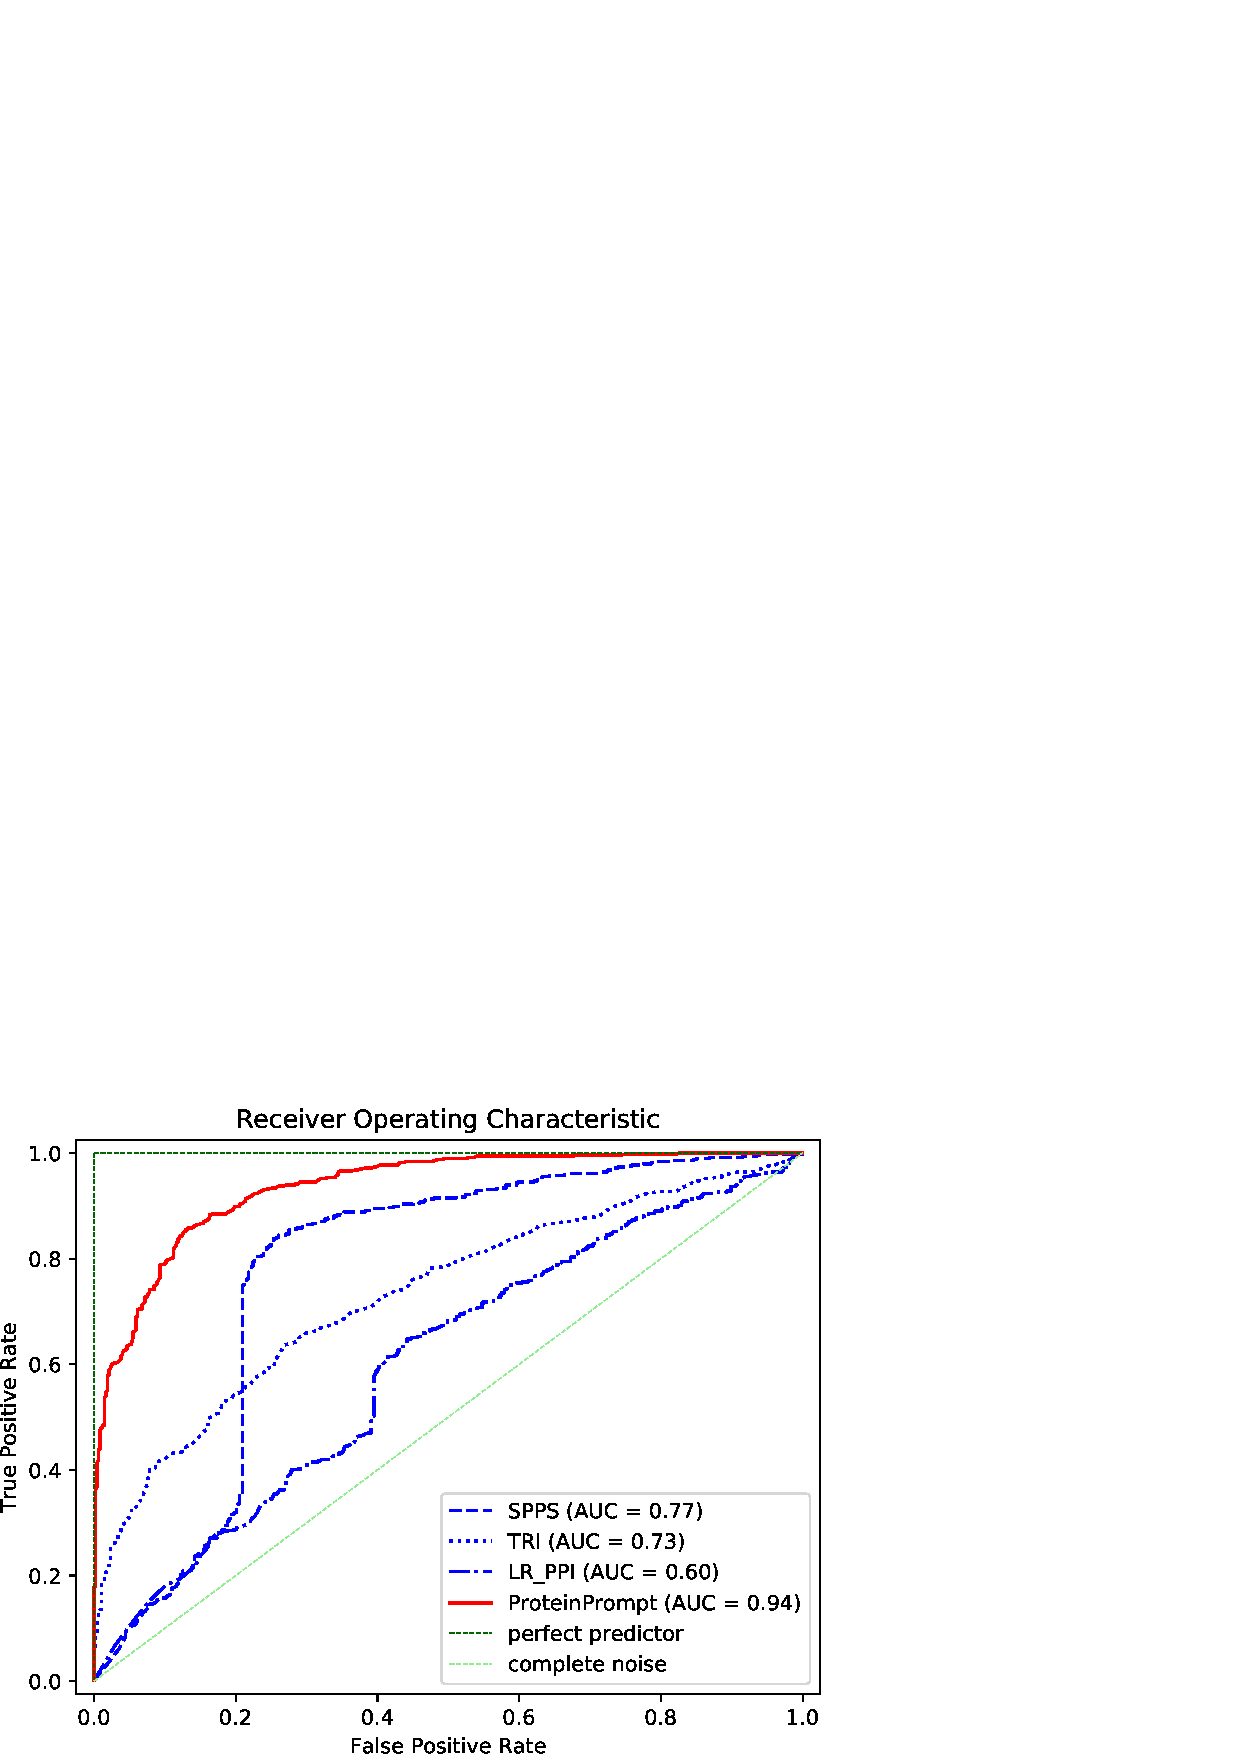
\includegraphics[width=0.5\textwidth]{img/comparison_roc.pdf}
  \caption{Comparison of ROC-curves between \tool, \spps, \tri, \lr\ 
    using a diminished test dataset including 968
    protein-protein pairs.}
  \label{fig:comparison}
\end{figure}


\begin{figure}
  \iffalse
%\documentclass{article}
%\usepackage{tikz}
%\usetikzlibrary{shapes.geometric, arrows}
%\usetikzlibrary{shapes.misc, positioning}
%
%\definecolor{lavander}{cmyk}{0,0.48,0,0}
%\definecolor{violet}{cmyk}{0.79,0.88,0,0}
%\definecolor{burntorange}{cmyk}{0,0.52,1,0}
%
%\def\lav{lavander!90}
%\def\oran{orange!30}
%
%\tikzstyle{neighbors}=[draw,circle,violet,bottom color=\lav,
%                  top color= white, font=\scriptsize,text=violet,minimum width=10pt]
%\tikzstyle{queries}=[draw,circle,burntorange, left color=\oran,
%                       text=violet,minimum width=30pt]
%
%\tikzstyle{io} = [trapezium, trapezium left angle=70, trapezium right angle=110, minimum width=3cm, minimum height=1cm, text centered, draw=black, color=burntorange,left color=\oran,text=black]
%
%\tikzstyle{res} = [trapezium, trapezium left angle=70, trapezium right angle=110, minimum width=3cm, minimum height=1cm, text centered, draw=black, color=violet,bottom color=\lav, top color=white,text=black]
%
%\tikzstyle{process} = [rectangle, minimum width=3cm, minimum height=1cm, text centered, draw=violet, bottom color=\lav, top color=white]
%
%\tikzstyle{grey} = [ rectangle, rounded corners=10pt, bottom color=black!10, top color=black!2] 
%
%\tikzstyle{aro} = [->, thick,  shorten >=2pt, shorten <=2pt]
%
%\begin{document}
\fi

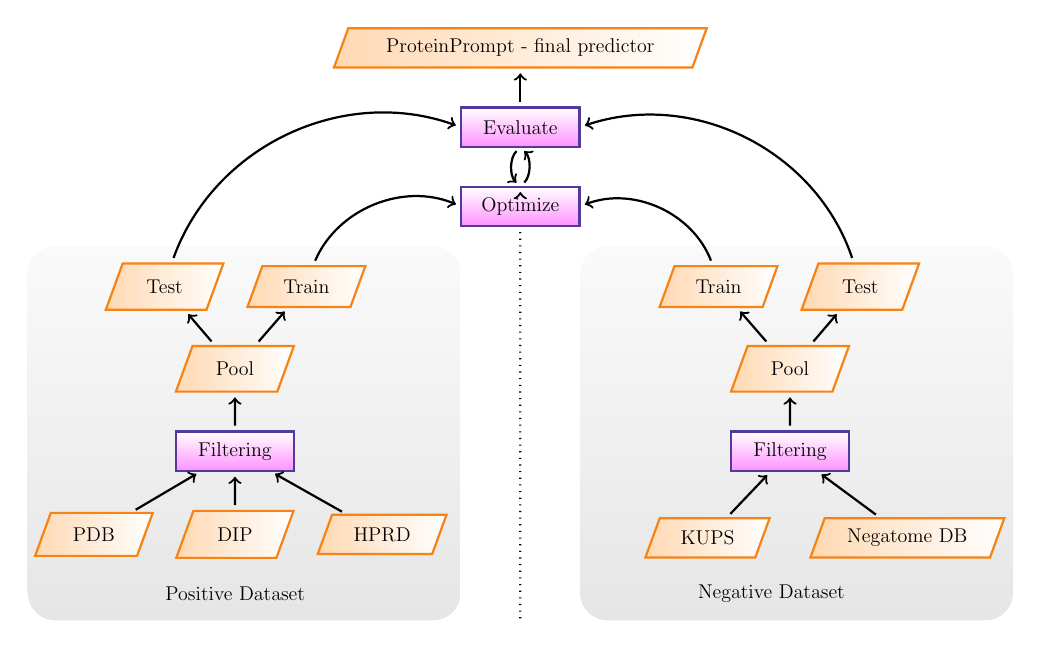
\begin{tikzpicture}[auto,thick, scale=0.5, transform shape,align=center, node distance = 1.5cm]

  \tikz {every node} = [font=\LARGE]
  
  \node (final) [io] { ProteinPrompt - final predictor};
  \node (apply) [process, below=1cm of final] {Evaluate}
  edge [aro] (final);
  \node (opt) [process,below=1cm of apply] {Optimize};

  \draw [aro,bend right=45] (apply.south) edge (opt.north)
                            (opt.north) edge (apply.south);


  \node[grey,minimum width=11cm,minimum height=9.5cm,below left=0.5cm and 0 of opt]{ \parbox[b][8.5cm]{4cm}{Positive Dataset}};
  
  \node (ptrain) [io,below left=1cm and 3.4cm of opt] {Train}
  edge[aro,bend left=45] (opt.west);

  \node (ptest)  [io,left=1cm of ptrain] {Test}
  edge[aro,bend left=45] (apply.west);

  \path (ptrain) -- node(ppool)[io,below=1.5cm]{Pool} (ptest);

  \draw [aro] (ppool) edge (ptest)
  edge( ptrain);

  \node (pclean) [process,below=1cm of ppool] {Filtering}
  edge[aro](ppool);
  
  
  \node (ip1) [io, below=1cm of pclean] {DIP}
  edge[aro](pclean);
  \node (ip2) [io,right=1cm of ip1] {HPRD}
  edge[aro](pclean);
  \node (ip3) [io,left=1cm of ip1] {PDB}
  edge[aro](pclean);

  \node[grey,minimum width=11cm,minimum height=9.5cm,below right=0.5cm and 0 of opt]{ \parbox[b][8.5cm]{5cm}{Negative Dataset}};

  \node (ntrain) [io,below right=1cm and 3cm of opt] {Train}
  edge[aro,bend right=45] (opt.east);

  \node (ntest)  [io,right=1cm of ntrain] {Test}
  edge[aro,bend right=45] (apply.east);

  \path (ntrain) -- node(npool)[io,below=1.5cm]{Pool} (ntest);

  \node (nclean) [process,below=1cm of npool] {Filtering}
  edge[aro] (npool);
  
  \draw [aro] (npool) edge (ntest)
  edge( ntrain);

  \node (ghost) [below=1.5cm of nclean]{};
  \node (in1) [io, right=0.5cm of ghost] {Negatome DB}
  edge[aro](nclean);
  \node (in2) [io, left=0.5cm of ghost] {KUPS}
  edge[aro](nclean);

  \draw [dotted, shorten <=2pt] (opt) edge (0,-14.6);
  
%  edge[aro, bend right=45] (ptest.north);

\end{tikzpicture}


%\end{document}

  

  \caption{Training of the learning algorithm: goal is to distinguish positive data of known binders from negative data of non-binders. Data from several sources was collected, such as ... Rigorous filtering is crucial for the quality of the data. In order to avoid overfitting, the datasets have to be split in training and testing data. In an iterative process the performance of the learning algorithm is maximized on the training dataset, while at the same time monitoring the performance on the testdata. }
\end{figure}


\begin{figure}
  \documentclass{article}
\usepackage{tikz}
\usetikzlibrary{shapes.geometric, arrows}
\usetikzlibrary{shapes.misc, positioning}

\definecolor{lavander}{cmyk}{0,0.48,0,0}
\definecolor{violet}{cmyk}{0.79,0.88,0,0}
\definecolor{burntorange}{cmyk}{0,0.52,1,0}

\def\lav{lavander!90}
\def\oran{orange!30}

\tikzstyle{neighbors}=[draw,circle,violet,bottom color=\lav,
                  top color= white, font=\scriptsize,text=violet,minimum width=10pt]
\tikzstyle{queries}=[draw,circle,burntorange, left color=\oran,
                       text=violet,minimum width=30pt]

\tikzstyle{io} = [trapezium, trapezium left angle=70, trapezium right angle=110, minimum width=3cm, minimum height=1cm, text centered, draw=black, color=burntorange,left color=\oran,text=black]

\tikzstyle{res} = [trapezium, trapezium left angle=70, trapezium right angle=110, minimum width=3cm, minimum height=1cm, text centered, draw=black, color=violet,bottom color=\lav, top color=white,text=black]

\tikzstyle{process} = [rectangle, minimum width=3cm, minimum height=1cm, text centered, draw=violet, bottom color=\lav, top color=white]

\tikzstyle{grey} = [ rectangle, rounded corners=10pt, bottom color=black!10, top color=black!2] 

\begin{document}
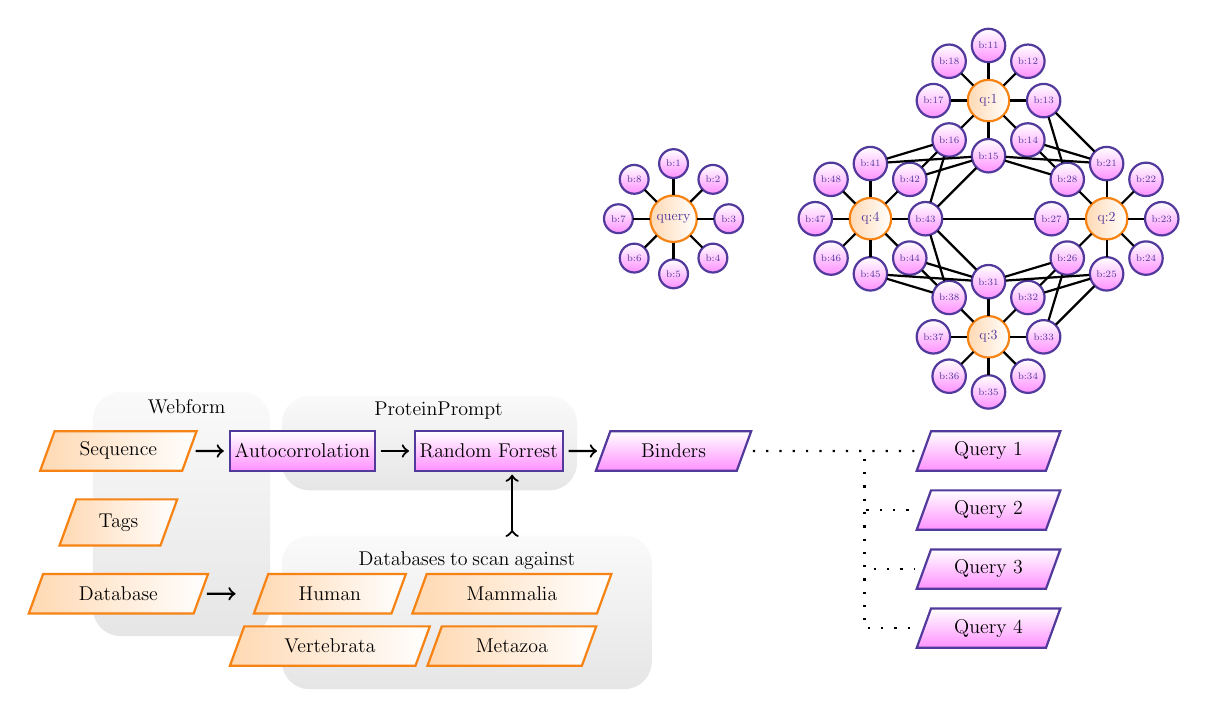
\begin{tikzpicture}[auto,thick, scale=0.5, transform shape,align=center, node distance = 1.5cm]

    \node[queries] (n0) at (-4,0) {query};
    \foreach \k/\l/\j in {1/1/2,-1/1/8,1.4/0/3,-1.4/0/7,1/-1/4,-1/-1/6,0/1.4/1,0/-1.4/5}{
        \node[neighbors] (n\j) at (\k-4,\l) {b:\j};
        %      \path (n\i\j) edge (\i);
        \draw (n\j) -- (n0);
    }
  \foreach \x/\y/\i in {1/0/4,7/0/2,4/3/1,4/-3/3} {
    \node[queries] (\i) at (\x,\y) {q:\i};
    \foreach \k/\l/\j in {1/1/2,-1/1/8,1.4/0/3,-1.4/0/7,1/-1/4,-1/-1/6,0/1.4/1,0/-1.4/5}{
        \node[neighbors] (\i\j) at (\x+\k,\y+\l) {b:\i\j};
        %      \path (n\i\j) edge (\i);
        \draw (\i\j) -- (\i);
    }
  }

  \foreach \i in {5,6}{
    \foreach \j in {1,2,3}{
      \draw (2\i) -- (3\j);
      \draw (1\i) -- (4\j);
    }
  }
  
  \foreach \i in {3,4,5}{
    \foreach \j in {1,8}{
      \draw (4\i) -- (3\j);
      \draw (1\i) -- (2\j);
    }
  }
  
  \draw (43) -- (27);


  

  \node (r1) [res, below of=35] {Query 1};
  \node (r2) [res, below of=r1] {Query 2};
  \node (r3) [res, below of=r2] {Query 3};
  \node (r4) [res, below of=r3] {Query 4};

  \node (webform) [grey, minimum width = 4.5cm, minimum height=6.2cm] at (-16.5cm,-7.5 ) {\parbox[t][5.8cm]{1.7cm}{\Large  Webform}};

  \node (server) [grey, minimum width = 7.5cm, minimum height=2.4cm] at (-10.2cm,-5.7 ) {\parbox[t][2.1cm]{2.8cm}{\Large  ProteinPrompt}};

  \node (result) [res] at (n5 |- r1) {Binders};

  \node (prompt) [process, left=1cm of result] {Random Forrest};

  \node (ac) [process, left=1cm of prompt] {Autocorrolation};

  \node (seq) [io, left=1cm of ac] {Sequence};
  \node (tag) [io, below=0.7 of seq] {Tags};
  \node (db)  [io, below=0.7 of tag] {Database};


  \node (backdb) [grey, minimum width=9.4cm, minimum height=3.9cm] at (-9.25cm,-10cm) {\parbox[t][3.1cm]{5.5cm}{\Large Databases to scan against}};
  
  \node (db1) [io, right=1.5cm of db] {Human};
  \node (db2) [io, right=0.5cm of db1] {Mammalia};
  \node (db3) [io, below=0.3cm of db1] {Vertebrata};
  \node (db4) [io, below=0.3cm of db2] {Metazoa};

  \draw [->, shorten >=2pt, shorten <=2pt] (seq) -- (ac);
  \draw [->, shorten <=2pt, shorten >=9pt] (db) -- (db1);
  \draw [->, shorten >=2pt, shorten <=2pt] (ac) -- (prompt);
  \draw [->, shorten >=2pt, shorten <=2pt] (prompt) -- (result);
  \draw [->, ] (-8.1,-7.9) edge (-8.1,-6.5);

  \draw [loosely dotted, shorten >=3pt, shorten <=3pt] (result) -- (r1);
  \draw [loosely dotted, shorten >=3pt] (0.85,-6.1) |- (r2);
  \draw [loosely dotted, shorten >=3pt] (0.85,-6.1) |- (r3);
  \draw [loosely dotted, shorten >=3pt] (0.85,-6.1) |- (r4);

  
  
\end{tikzpicture}
\end{document}

  \caption{The user has to provide the query sequence, a tag for later identification, and to select the database in which potential binders are expected. \tool converts the sequence first into autocorrelation descriptors prior to calling the random forrest algorithm. The server returns a list of potential binders, sorted by expected binding strength. The website displays a searchable and filterable table. Additionally a download link is provided. Having accumulated the lists for several queries, connectivities, and thus complex binding networks can be investigated. }
\end{figure}



%% Here is the endmatter stuff: Supplementary Info, etc.
%% Use \item's to separate, default label is "Acknowledgements"

%\begin{addendum}
% \item Put acknowledgements here.
% \item[Competing Interests] The authors declare that they have no
%competing financial interests.
% \item[Correspondence] Correspondence and requests for materials
%should be addressed to R.S. and S.C. (email: rene.staritzbichler@medizin.uni-leipzig.de,sebastian@bioinf.uni-leipzig.de).
%\end{addendum}




\end{document}


